\section{Anexos}
\vspace*{2cm}

\subsection*{Anexo 1: Diagrama de flujo}
\begin{figure}[H]
	\centering
	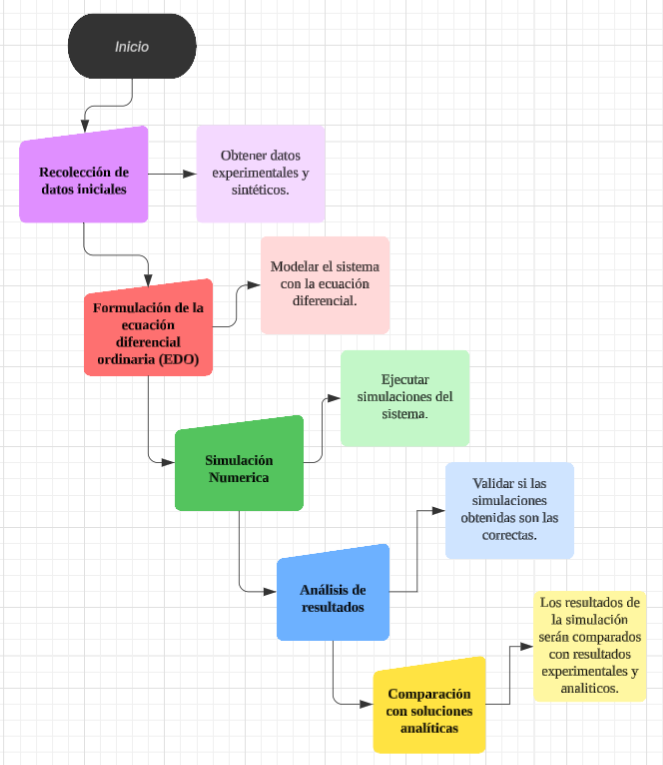
\includegraphics[width=0.8\textwidth]{5.png}
	\caption{Diagrama de flujo metodológico}
\end{figure}

\newpage

\subsection*{Anexo 2: Código y gráfica de la carga en el capacitor vs. Tiempo}
\begin{figure}[H]
	\centering
	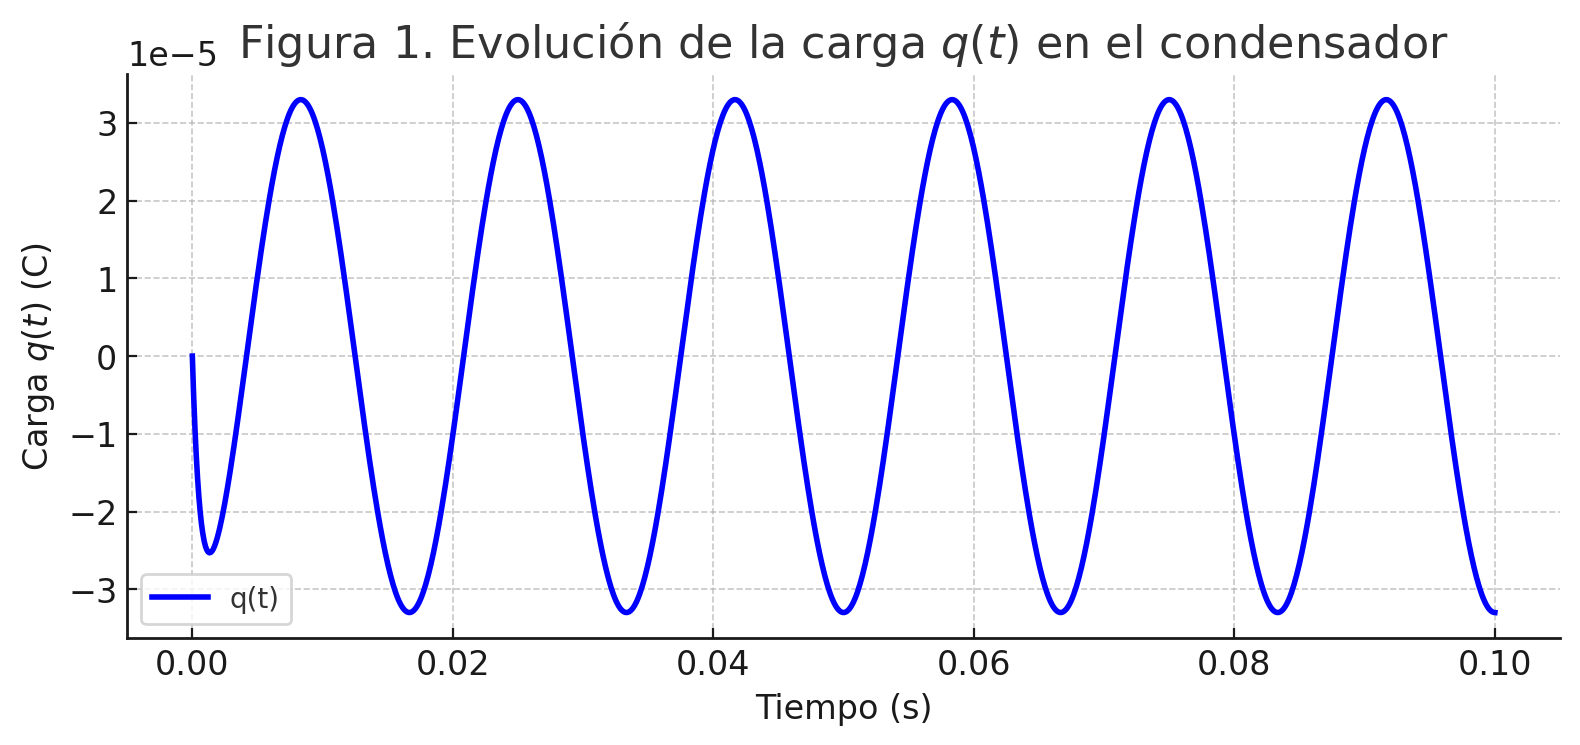
\includegraphics[width=0.8\textwidth]{7.png}
	\caption{Carga del capacitor vs. tiempo}
\end{figure}

\begin{lstlisting}[language=Python, caption={Código Python para simulación de carga}, label={cod:carga}, frame=single, basicstyle=\footnotesize\ttfamily]
import numpy as np
import matplotlib.pyplot as plt

R_bat = 1.2
R_x = 0.1
R_c = 0.3
C = 1000e-6
omega = 2 * np.pi * 60

tau = C * (R_bat + R_x + R_c)

A = 3.2982e-5
B = 5.4679e-8
C_p = -3.2982e-5

t = np.linspace(0, 0.1, 1000)
q_t = A * np.exp(-t / tau) + B * np.sin(omega * t) + C_p * np.cos(omega * t)

plt.figure(figsize=(8, 4))
plt.plot(t, q_t, label='q(t)', color='blue', linewidth=2)
plt.title('Carga en el Capacitor vs. Tiempo')
plt.xlabel('Tiempo (s)')
plt.ylabel('Carga q(t) (C)')
plt.grid(True)
plt.legend()
plt.tight_layout()
plt.show()
\end{lstlisting}

\newpage

\subsection*{Anexo 3: Código y gráfica del análisis espectral de la señal q(t) mediante FFT}
\begin{figure}[H]
	\centering
	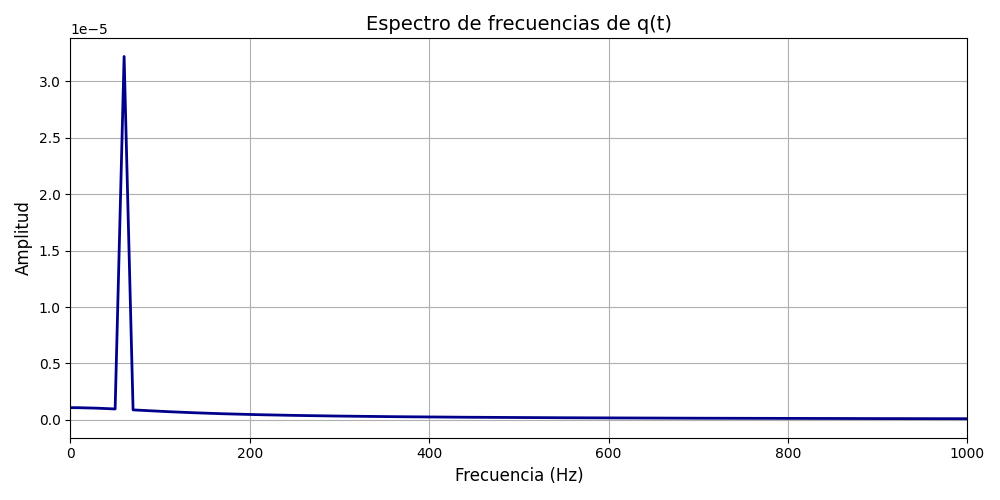
\includegraphics[width=0.8\textwidth]{8.png}
	\caption{Espectro de frecuencias de la señal q(t)}
\end{figure}

\begin{lstlisting}[language=Python, caption={Código Python del análisis espectral}, label={cod:fft}, frame=single, basicstyle=\footnotesize\ttfamily]
import numpy as np
import matplotlib.pyplot as plt
from scipy.fft import fft, fftfreq

tau = 1.6e-3
omega = 2 * np.pi * 60
f_s = 10000
T = 1 / f_s
t = np.arange(0, 0.1, T)

A = 3.2982e-5
B = 5.4679e-8
C = -3.2982e-5


N = len(t)
yf = fft(q_t)
xf = fftfreq(N, T)[:N//2]
amplitud = 2.0 / N * np.abs(yf[0:N//2])

plt.figure(figsize=(10, 5))
plt.plot(xf, amplitud, color='darkblue', linewidth=2)
plt.title('Espectro de frecuencias de q(t)', fontsize=14)
plt.xlabel('Frecuencia (Hz)', fontsize=12)
plt.ylabel('Amplitud', fontsize=12)
plt.grid(True)
plt.xlim(0, 1000)
plt.tight_layout()
plt.show()
\end{lstlisting}

